\documentclass[11pt]{article}
\usepackage[a4paper,margin=22mm,headheight=16pt]{geometry}
\usepackage{fontspec,xeCJK,xcolor,graphicx,enumitem,fancyhdr,titlesec}
\usepackage{hyperref}
\IfFontExistsTF{Times New Roman}{\setmainfont{Times New Roman}}{\setmainfont{TeX Gyre Termes}}
\IfFontExistsTF{FangSong}{\setCJKmainfont[AutoFakeBold=2]{FangSong}}{\IfFontExistsTF{仿宋}{\setCJKmainfont[AutoFakeBold=2]{仿宋}}{\IfFontExistsTF{FandolFang-Regular.otf}{\setCJKmainfont[AutoFakeBold=2]{FandolFang-Regular.otf}}{\setCJKmainfont{FandolSong-Regular.otf}}}}
\definecolor{ink}{HTML}{173747}\definecolor{accent}{HTML}{227E82}
\hypersetup{colorlinks=true,urlcolor=accent,linkcolor=accent}
\linespread{1.22}\setlength{\parindent}{0pt}\setlength{\parskip}{6pt}
\setlist[itemize]{leftmargin=1.4em,itemsep=3pt}
\titleformat{\section}{\large\bfseries\color{ink}}{}{0pt}{}
\titlespacing*{\section}{0pt}{14pt}{7pt}
\pagestyle{fancy}\fancyhf{}\lhead{\small OMNI LEARNING / Learning guide}\rhead{\small Source-grounded learning}\cfoot{\small\thepage}
\emergencystretch=2em\widowpenalty=10000\clubpenalty=10000
\newcommand{\Needspace}[1]{\par\begingroup\dimen0=#1\relax\vskip0pt plus\dimen0\penalty-100\vskip0pt plus-\dimen0\vskip\dimen0\penalty9999\vskip-\dimen0\vskip0pt\endgroup}
\begin{document}


{\LARGE\bfseries\color{ink} Understand the Night Sky While Traveling}\par

2026-10-09 | Learning plan / 3 days\par\vspace{6pt}

\Needspace{5\baselineskip}\section*{Your starting point and boundaries}

This English course is for a complete beginner traveling in China, using the naked eye and a phone star chart. It covers general principles for city and rural skies. No telescope, purchased app, astronomy mathematics or prior constellation knowledge is required. A phone chart can help identify visible objects, but equipment is not essential for starting skywatching. [S1]

Three short lessons build a practical framework. They do not promise that a named planet, constellation or the Milky Way will be visible on a particular trip. Exact visibility depends on place, date, time, sky conditions and the horizon.

\Needspace{5\baselineskip}\section*{What you will be able to do}

Identify: check a bright point against a correctly configured chart and explain why a visual clue is provisional. Stars commonly twinkle because of atmospheric turbulence; the light from a planet tends to average those effects. [S2]

Explain: describe Moon phases as our changing view of the sunlit half, rather than ordinary phases being caused by Earth blocking the light. [S3]

Plan: choose a target, a suitable site and viewing window, and a weather fallback. The overview below shows the sequence: identification gives you a target; the Moon model helps you consider timing and sky brightness; both feed the outing plan. Its Moon icons illustrate changing appearance, not orbital geometry.

\begin{center}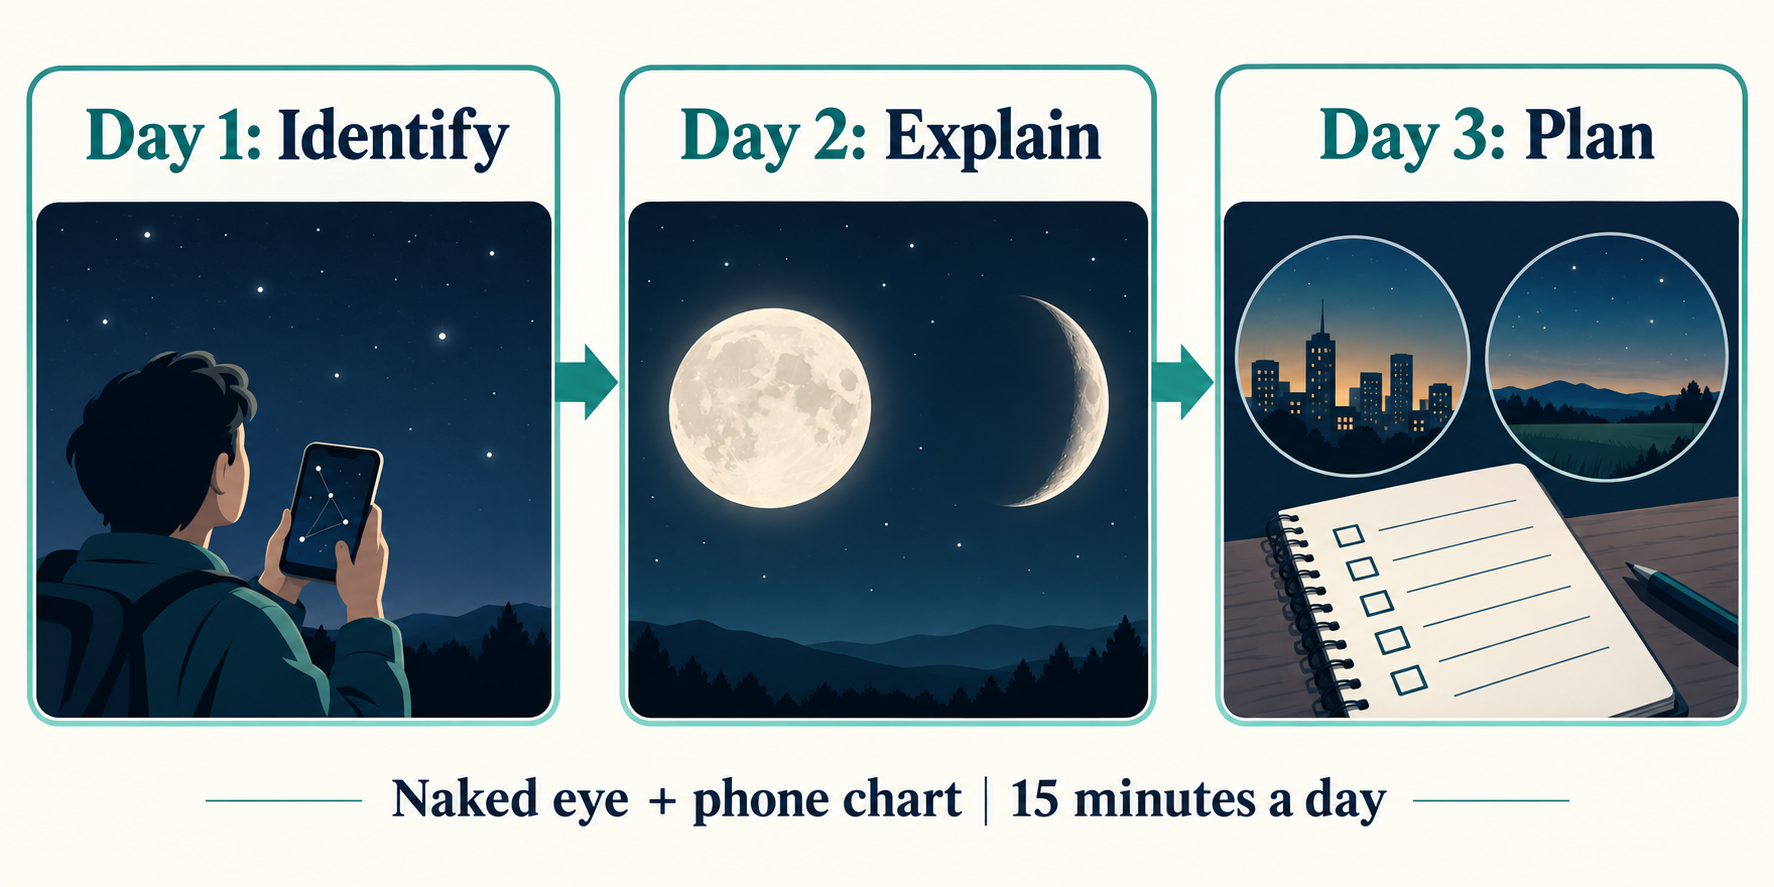
\includegraphics[width=\linewidth,height=0.26\textheight,keepaspectratio]{../assets/figure-8540a079e446.png}\par

{\small Course route: identify a target, explain the Moon, then plan an outing. The full and crescent Moon icons are alternative appearances, not two Moons seen together; no dated sky map is shown.}\par

{\footnotesize AI-generated teaching illustration, created with the host image-generation tool. Prompt and provenance retained locally; not observational evidence.}\end{center}

\Needspace{5\baselineskip}\section*{Schedule and the 15-minute workload}

Day 1, Day 2 and Day 3 run in order, with weekends included: 45 minutes of core study in total. Nominal generation start: 10:00, Asia/Shanghai. This is a sample acceptance course; the time is metadata only and no live schedule will be created. If used as a generation trigger, 10:00 would start research and rendering; delivery would follow inspection, rather than occur at a guaranteed 10:00.

Each lesson uses 2 minutes of recall or baseline questions, 8 minutes of reading and figure study, and 5 minutes of practice plus self-check. These are estimates, not measured learner reading times. Required tasks can be completed indoors. Outdoor observing and all expansion links are optional, outside the 15-minute budget. Full dark adaptation may take half an hour or more. [S5]

\Needspace{5\baselineskip}\section*{Day 1 — Stars or Planets? Read the Sky with a Phone Chart}

Start with the horizon, direction and height above it. Learn the difference between identifying a point by appearance and confirming it by its position on a chart. Twinkling is a useful clue, not a sufficient classification rule. [S2] A chart must match the observing location, date and time, and can show objects that are not actually visible. [S4]

Core practice: use your chart indoors to select one star and one planet, read their categories and record their displayed direction and height, or below-horizon status. This rehearses the method; it is not a forecast for a trip. If the app is unavailable, use a clearly labeled teaching example in the lesson.

Output: a two-row identification note plus one sentence explaining why a steady point still needs checking. Self-check criterion: correct object category and chart context, with uncertainty stated. Baseline recall asks what you currently think makes a point a planet; no prior lesson is needed. Bridge: the Moon is another reflected-light object, but its changing shape needs a geometry model.

\Needspace{5\baselineskip}\section*{Day 2 — Moon Phases: Sunlight and Our Changing View}

First retrieve Day 1: explain why twinkling is a clue rather than proof. Then follow sunlight, the Moon and the observer in a simplified lit-half model. Identify new, quarter and full Moon; use waxing and waning for increasing and decreasing visible illumination. Ordinary phases differ from lunar eclipses. Approximate rise/set patterns are guides, not exact local times. [S3]

Core practice: study the lesson figure, explain three phases in your own words, then use a desk lamp and a ball if available, or the supplied paper model. Never use the real Sun for the exercise. Compare an evening quarter-Moon observation with a full-Moon night as two hypothetical choices.

Output: a three-sentence phase explanation and a reason Moon viewing and faint-star viewing can favor different conditions. Self-check criterion: the model changes how much of the lit half we see, without invoking Earth’s shadow for normal phases. Bridge: Moon brightness and whether it is above the horizon become inputs to your outing plan. [S5]

\Needspace{5\baselineskip}\section*{Day 3 — Plan a Simple City or Rural Stargazing Outing}

Retrieve Days 1 and 2 without looking: how would you verify a bright point, and what causes ordinary Moon phases? Combine those answers with site conditions. City glow hides fainter targets; a rural location can offer darker skies, but clouds, bright Moonlight and blocked horizons still matter. [S1] [S5]

Core practice: write a six-part outing card: (1) target and purpose; (2) chart location/date/time and target direction/height; (3) Moon phase and local rise/set checks; (4) cloud/weather and clear horizon checks; (5) site access, return route and phone-light preparation; (6) a fallback if conditions fail. No specific travel date or visibility prediction is required.

Output: one hypothetical city plan, then two justified rural adjustments. Self-check criterion: choose bright, chart-confirmed targets for the city; justify rural darkness and horizon choices without guaranteeing a richer view. The card must include a condition for postponing or changing the activity. Local access and weather must be checked again before any real outing. [S5]

\Needspace{5\baselineskip}\section*{Assessment, feedback and revisions}

At the end of Day 3, use three checks: can you verify an object category with chart context, explain phases without the Earth-shadow misconception, and complete all six parts of the outing card? Aim for all three; this is a course assessment choice, not a validated mastery score. Each lesson will include a worked example and self-check answers.

If a check fails, revisit that lesson’s figure and retry the specific task. The opening recall in Days 2 and 3 supplies spaced review within this short course. You can submit answers or describe confusing steps for feedback; absence of a response will not be recorded as learning. Optional field observations test transfer, but are not required for completion.

This plan awaits your explicit approval. Day 01 is requested immediately after approval; it has not been created. If the plan needs changes, preserve this version and render a revised course version for approval.

\Needspace{5\baselineskip}\section*{Evidence and practical limits}

The links below were searched and opened for this plan. Their foundations are stable; chart controls, site access and local conditions can change. No phone app was operated or China network access tested. If a listed website is unavailable during travel, use the same setting checks in your existing chart. The diagram is an AI-generated teaching illustration, not observational evidence or an official NASA figure. Research records and image provenance accompany the plan. This independently authored course is not reviewed or endorsed by the source publishers.

\Needspace{6\baselineskip}\section*{Further reading}\small Optional; outside the daily core time budget.\begin{enumerate}[leftmargin=1.6em]

\item [S1] \href{https://science.nasa.gov/skywatching/faq/}{Skywatching FAQ} — Read General Questions for naked-eye tools and light pollution; Moon and Planets for visibility basics. Page last updated 2024-09-03.\par NASA Science | Published: Not stated | Checked: 2026-10-09

\item [S2] \href{https://imagine.gsfc.nasa.gov/ask\_astro/night\_sky.html}{Why do stars twinkle while planets usually look steady?} — Find the twinkling answer by Koji Mukai and Maggie Masetti, question submitted 1998-12-17. Use the atmospheric explanation; unrelated old links are not required.\par NASA Goddard, Imagine the Universe! | Published: Not stated | Checked: 2026-10-09

\item [S3] \href{https://science.nasa.gov/moon/moon-phases/}{Moon Phases} — Read All Moon Phases and Daytime Moons. Connect the changing view of the lit half to approximate viewing times. Updated 2026-08-03; exact times need local data.\par NASA Science | Published: Not stated | Checked: 2026-10-09

\item [S4] \href{https://www.timeanddate.com/astronomy/night/help}{How to Use the Night Sky Map} — Read location selection, object selection and tracking. Use the workflow with your existing chart; this service is an optional example, not a required app.\par timeanddate.com | Published: Not stated | Checked: 2026-10-09

\item [S5] \href{https://science.nasa.gov/solar-system/how-to-find-good-places-to-stargaze/}{How to Find Good Places to Stargaze} — Read weather, Moon phase, landscape and arrival sections to build an outing checklist. Last updated 2024-11-04. Use local Moon rise/set data, not a fixed date rule.\par NASA Science | Published: Not stated | Checked: 2026-10-09

\end{enumerate}

\end{document}